\section{Experimental Design}

\label{sec:evaluation}

To evaluate our strategy, in this section we present the empirical study we conduct. Before explaining our study, we first introduce the terminology we use throughout this paper. In particular, we define in what follows four categories: abort, skip, fail, and pass.

\begin{itemize}

	\item \textbf{Abort:} students that aborted the course before the final exam;
	\item \textbf{Skip:} students allowed to do the final exam but did not show up;
	\item \textbf{Fail:} students who failed the course;
	\item \textbf{Pass:} students who successfully passed the course.

\end{itemize}

Now, we present the objetives and hypothesis (Section~\ref{sec:hypotheses}) of our study, then the participants and material (Section~\ref{sec:participants}) we use, and finally we detail the procedure (Section~\ref{sec:procedure}) we use during the evaluation.

\subsection{Objective and Hypothesis}

\label{sec:hypotheses}

The objective of this study is to evaluate to what extent our strategy is capable of identifying potential failing students. This way, based on this objective, our hypothesis is the following: In the first 30 days, students with lower number of submissions and correct submissions tend to fail the course. \todo{Essa hipotese esta errada. Ja deveriamos colocar 72\%?}

\subsection{Participants and Material}

\label{sec:participants}

The participants of our study consist of students of introductory programming courses at the Federal University of Alagoas, Brazil. We ministered these courses during 3.5 years and collected the metrics we detail in Section~\ref{sec:metrics} of each student by using Huxley. The professor informed all students that the use of Huxley was mandatory during the courses, i.e., for applying exercises and formal exams. Table~\ref{tab:participants} distribute the number of participants per semester.

\begin{table}[h]
\centering
\begin{tabular}{|c|c|}
\hline
\textbf{Course} & \textbf{Number of enrolled students}\\ \hline
2010.02 & 32\\ \hline
2011.01 & 38\\ \hline
2011.02 & 35\\ \hline
2012.01 & 34\\ \hline
2012.02 & 29\\ \hline
2013.01 & 28\\ \hline
2013.02 & 31\\ \hline
\textbf{TOTAL:} & \totalStudents\\ \hline
\end{tabular}
\caption{Participants per course.}
\label{tab:participants}
\end{table}

The material of this study consists of almost 300 programming exercises in Huxley. They were available for all students of all courses we use in this paper.

\subsection{Procedure}

\label{sec:procedure}

Figure~\ref{fig:procedure} illustrates how we perform our evaluation. The result of executing our strategy consists of groups of students according to the clustering algorithm (here we use k-means). Now, according to the groups, we have the potential failing students. These students are the ones that have a small number of submissions and correct submissions (represented by circles). Notice we also have students that are potential candidates to successfully pass (represented by stars): due to the high number of submissions to Huxley after 30 days, they seem to be practicing programming really hard. Depending on the number of groups we set to k-means, in Figure~\ref{fig:procedure} we have three, we have the intermediary students (represented by squares).

\begin{figure}[htb]
\centering
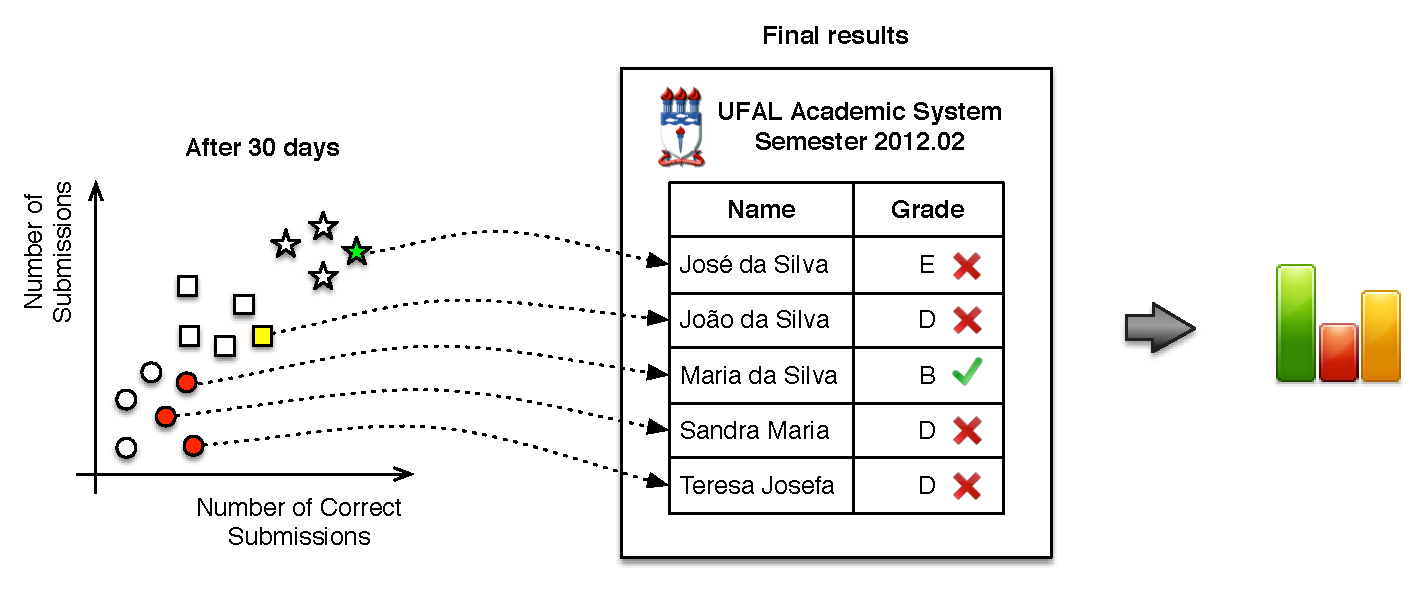
\includegraphics[width=1.0\textwidth]{images/Procedure.pdf}
\caption{Checking the strategy results against the actual grades.}
\label{fig:procedure}
\end{figure}

After applying the strategy, we now need to check whether it correctly predicts the failing students after 30 days. To do so, we use the academic system of the Federal University of Alagoas to look for grades and check whether the students failed or not. For example, for the detached circles, the strategy successfully identified that, after 30 days, two students would not pass and they indeed did not. Notice, however, that we may face false positives. Despite indicating the student \textit{Maria da Silva}\footnote{All names we consider in this paper are fictitious.} as a failing one after 30 days, such a student seemed to improve herself during the semester and she has been approved. In addition, we may also face false negatives. For instance, our strategy does not point the students \textit{Jos\'{e} da Silva} and \textit{Jo\~{a}o da Silva} as failing ones. Although \textit{Jos\'{e} da Silva} seems to be one of the best students after 30 days, he failed the course. The several reasons why this happened is out of the scope of this paper.

To better structure and analyze our results and, at the same time, take false positives and false negatives into account, we consider the following two metrics: precision and recall. Precision is the fraction of retrieved students that are relevant, i.e., the students pointed by the strategy that indeed failed the course. We have a perfect precision, 1.0, when every student retrieved by the strategy is relevant (i.e., a failing student), which means we have no false positives. Precision focuses on \textit{quality} and \textit{accuracy}. However, the precision says nothing about whether \textit{all} relevant students were indeed retrieved.

\vspace{0.1cm}
$$
Precision = \frac{| \{relevant\_students\} \cap \{retrieved\_students\} |}{| \{retrieved\_students\} |}
$$
\vspace{0.1cm}

Recall, in its turn, is the fraction of relevant students that are retrieved, i.e., it is the probability of retrieving a failing student. A perfect recall, 1.0, means that we retrieve all failing students, which means we have no false negatives. In this context, recall focuses on \textit{completeness} and \textit{quantity}. Notice that recall says nothing about how many irrelevant students (students that will pass) the strategy retrieved.

\vspace{0.1cm}
$$
Recall = \frac{| \{relevant\_students\} \cap \{retrieved\_students\} |}{| \{relevant\_students\} |}
$$
\vspace{0.1cm}

To better explain these metrics, consider the detached students in Figure~\ref{fig:procedure} as our set (three circles, one square, and one star). The relevant set is \textit{\{Jos\'{e}, Jo\~{a}o, Sandra, Teresa\}}, whereas the retrieved set is \textit{\{Maria, Sandra, Teresa\}}. The intersection set is \textit{\{Sandra, Teresa\}}. This way, we have

\vspace{0.2cm}
\noindent
\scriptsize
\begin{minipage}{.5\linewidth}
\centering
$$
Precision = \frac{|\{Sandra, Teresa\}|}{|\{Maria, Sandra, Teresa\}|} = 67\%;
$$
\end{minipage}
\begin{minipage}{.5\linewidth}
$$
Recall = \frac{|\{Sandra, Teresa\}|}{|\{\textit{\text{Jos\'{e}}}, \textit{\text{Jo\~{a}o}}, Sandra, Teresa\}|} = 50\%.
$$
\end{minipage}
\normalsize
\vspace{0.2cm}

Our strategy pointed two out of three students as failed ones and they indeed failed. Therefore, we have 67\% of accuracy when identifying potential failing students, raising one false positive. On the other hand, only two out of four students have been pointed as failed ones. This means that the strategy was not able to identify all failing students, raising two false negatives.

Last but not least, after confronting the strategy results with the academic system and summarizing precision and recall, we apply a statistical test to check for significance. Here, we rely on the proportion statistical test based on the Bernoulli distribution~\cite{} so that we have a binary distribution: fail or pass.

\section{Results and Discussion}

In this section, we describe the results and test our hypotheses before discussing their implications. All data, materials, and R scripts are available at \url{http://www.ic.ufal.br/}.

\subsection{Results}

In our evaluation, we use data of 7 courses (3.5 years) totalling \totalStudents students. We apply our strategy by setting k-means to compute two and three groups. We now proceed separately, reporting the results considering both cases.

\subsubsection{Two groups}

When considering two groups, we set the strategy to consider all students in two categories: fail or pass. Figure~\ref{fig:2-groups} illustrates the results for all courses. Notice that Figure~\ref{fig:2-2011-01} contains an outlier. In this particular case, the strategy pointed that all students but one would fail the course. This way, this represents a disadvantage of using two groups.

\begin{figure*}[ht]
     \begin{center}
         \subfigure[2010.02] {
             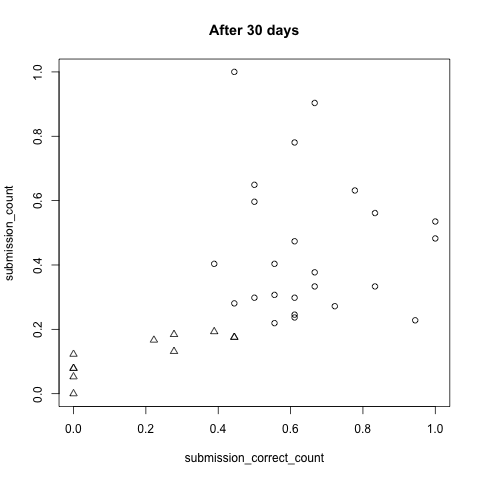
\includegraphics[scale=0.21]{images/2-2010-02.png}
             \label{fig:2-2010-02}
         }
         \subfigure[2011.01] {
             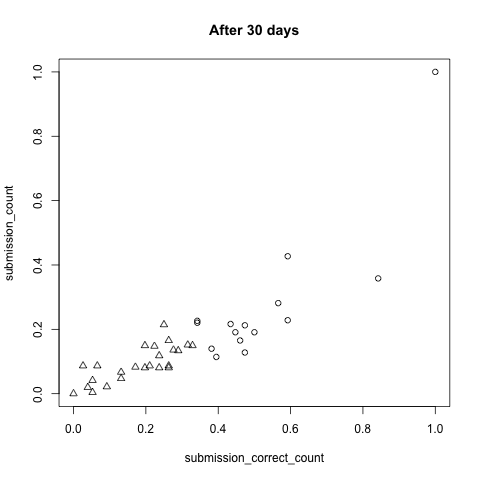
\includegraphics[scale=0.21]{images/2-2011-01.png}
             \label{fig:2-2011-01}
         }
         \subfigure[2011.02] {
             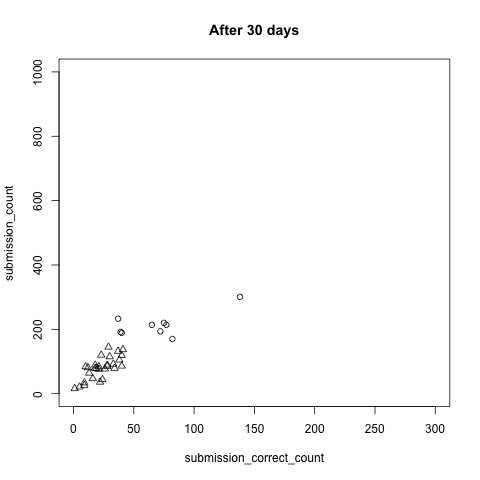
\includegraphics[scale=0.21]{images/2-2011-02.png}
             \label{fig:2-2011-02}
         }
         \subfigure[2012.01] {
             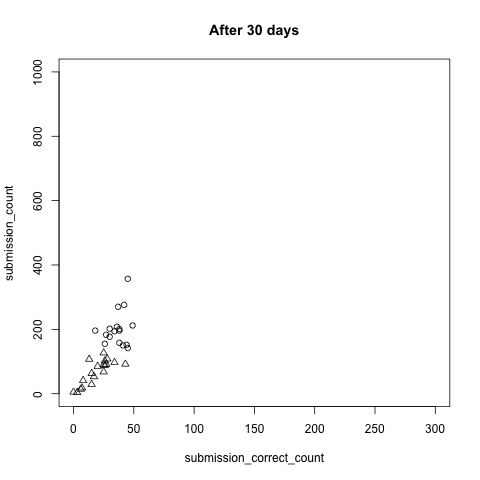
\includegraphics[scale=0.21]{images/2-2012-01.png}
             \label{fig:2-2012-01}
         }
         \subfigure[2012.02] {
             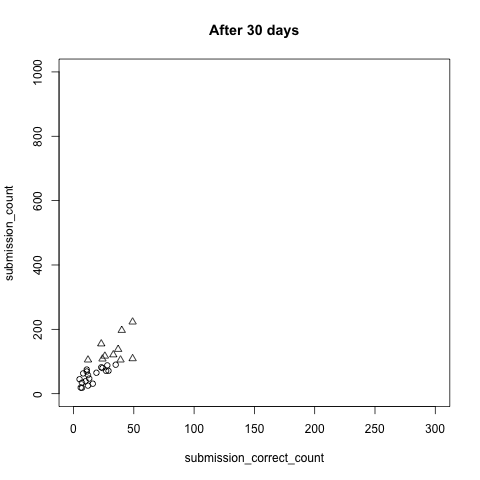
\includegraphics[scale=0.21]{images/2-2012-02.png}
             \label{fig:2-2012-02}
         }
         \subfigure[2013.01] {
             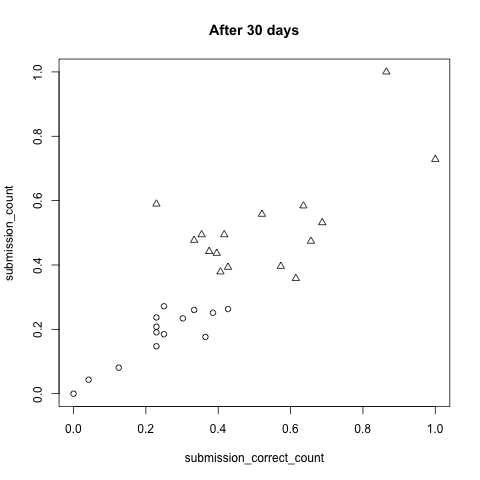
\includegraphics[scale=0.21]{images/2-2013-01.png}
             \label{fig:2-2013-01}
         }
         \subfigure[2013.02] {
             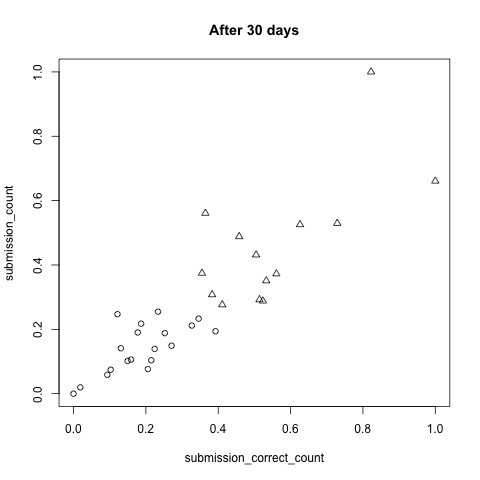
\includegraphics[scale=0.21]{images/2-2013-02.png}
             \label{fig:2-2013-02}
         }
     \end{center}
     \caption{Strategy applied with two groups.}
	 \label{fig:2-groups}
\end{figure*}

By using two groups, we achieve the following results for precision and recall:

\vspace{0.2cm}
\noindent
\begin{minipage}{.5\linewidth}
\centering
$$
Precision = \frac{92}{145} = 63\%;
$$
\end{minipage}
\begin{minipage}{.5\linewidth}
$$
Recall = \frac{92}{115} = 80\%.
$$
\end{minipage}
\vspace{0.2cm}

Besides these disadvantages, our strategy is susceptible to blablabla, raising outliers.

\subsubsection{Three groups}

Analogously, we set our strategy to consider three groups. Here, besides the failing and passing groups, there is one extra group where the strategy cannot conclude anything about it. Figure~\ref{fig:3-groups} shows the results for three groups. Differently from two groups, here outliers do not compromise the strategy.

%\begin{figure*}[h]
%     \begin{center}
%         \subfigure[2010.02] {
%             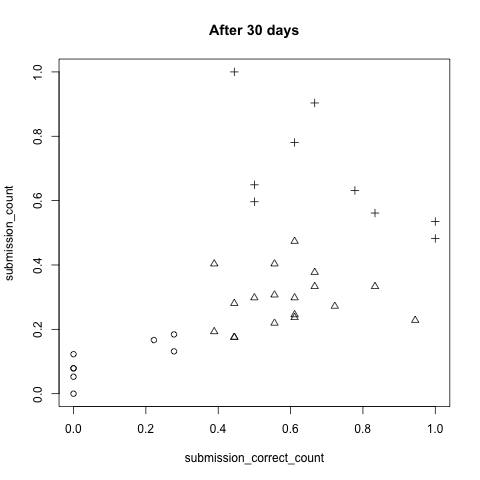
\includegraphics[scale=0.21]{images/3-2010-02.png}
%             \label{fig:3-2010-02}
%         }
%         \subfigure[2011.01] {
%             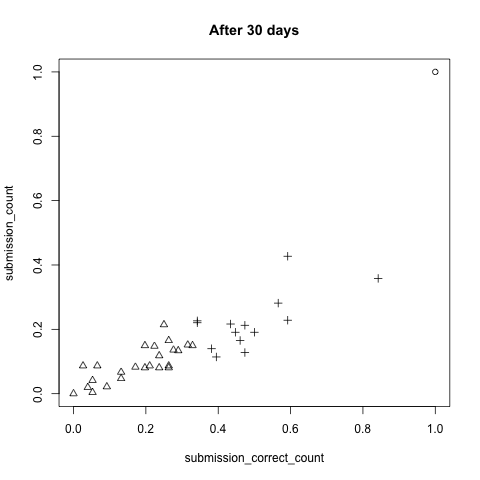
\includegraphics[scale=0.21]{images/3-2011-01.png}
%             \label{fig:3-2011-01}
%         }
%         \subfigure[2011.02] {
%             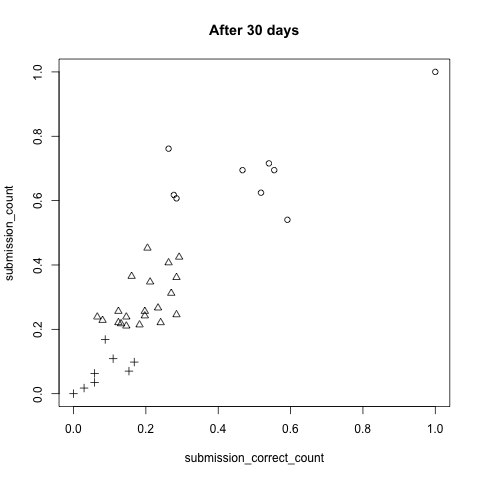
\includegraphics[scale=0.21]{images/3-2011-02.png}
%             \label{fig:3-2011-02}
%         }
%         \subfigure[2012.01] {
%             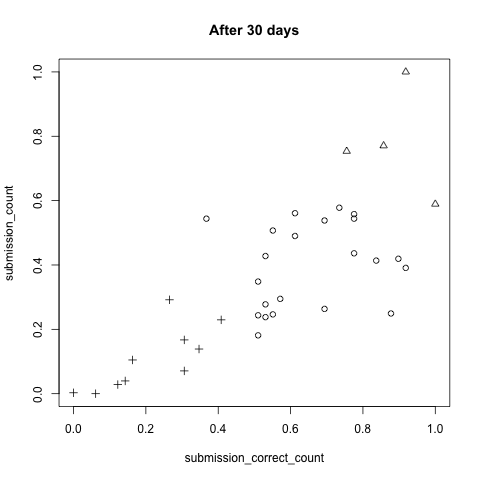
\includegraphics[scale=0.21]{images/3-2012-01.png}
%             \label{fig:3-2012-01}
%         }
%         \subfigure[2012.02] {
%             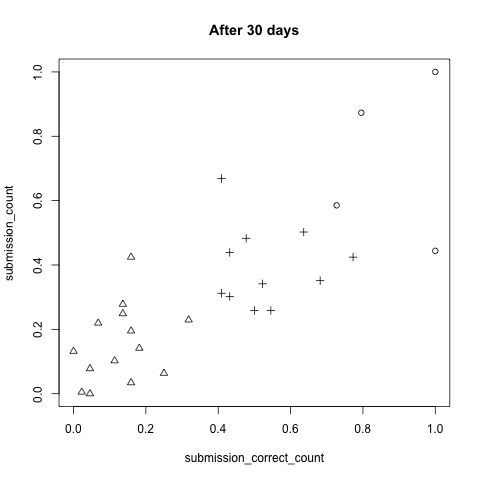
\includegraphics[scale=0.21]{images/3-2012-02.png}
%             \label{fig:3-2012-02}
%         }
%         \subfigure[2013.01] {
%             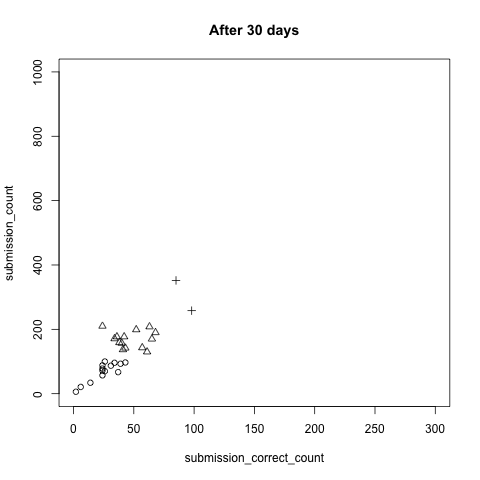
\includegraphics[scale=0.21]{images/3-2013-01.png}
%             \label{fig:3-2013-01}
%         }
%         \subfigure[2013.02] {
%             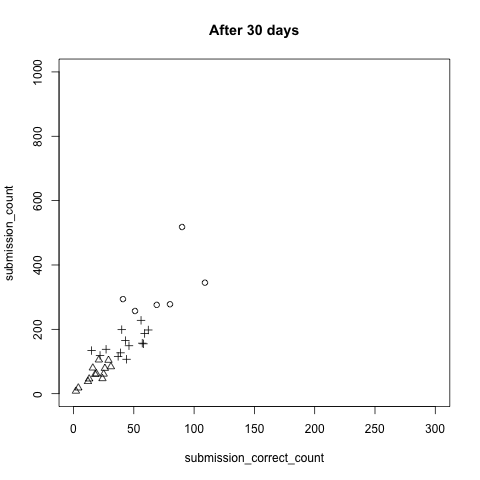
\includegraphics[scale=0.21]{images/3-2013-02.png}
%             \label{fig:3-2013-02}
%         }
%     \end{center}
%     \caption{Strategy applied with three groups.}
%	 \label{fig:3-groups}
%\end{figure*}

We present the precision and recall for three groups in what follows:

\vspace{0.2cm}
\noindent
\begin{minipage}{.5\linewidth}
\centering
$$
Precision = \frac{73}{91} = 80\%;
$$
\end{minipage}
\begin{minipage}{.5\linewidth}
$$
Recall = \frac{73}{115} = 63\%.
$$
\end{minipage}
\vspace{0.2cm}

\begin{itemize}

	\item Os graficos para 3 grupos est�o coloridos e nao tem formas (triangulo, circulo etc). Se gerarmos de novo vai alterar todos os resultados.

	\item \todo{Caralho, que negocio louco da porra. Com 2 grupos, temos 63 e 80. Com 3 grupos e exatamente o contrario, precision com 80 e recall com 63.}

	\item \todo{Falar sobre os resultados do teste de hipotese}

	\item \todo{Olhar se, para os alunos onde o algoritmo errou, eles foram pra prova final. Para tres grupos, alguma relacao com o grupo do meio?}

\end{itemize}

\subsection{Discussion}

\begin{itemize}

	\item \todo{3 grupos: Voce realmente deve prestar atencao nos alunos que ela retornou, pq ela acerta com 72\% de certeza. Mas devemos tambem ficar atentos, pois ela deixa muita gente de fora, pois a certeza do recall � de apenas 55\%}
	\item \todo{2 grupos: Ela erra muito, pois o precision foi muito baixo. Embora o recall tenha sido alto, isso significa que a estrategia esta retornando gente demais, incluindo os que deveriam retornar.}
	\item \todo{Sendo assim, acho que para o professor a estrategia com 3 grupos e mais util, pois ele podera focar naquele subconjunto que a certeza de estarem com problemas realmente e grande.}
	\item \todo{Discutir os resultados em relacao a prova final. Ainda nao computamos isso. Mais alguma outra coisa neste sentido que poderiamos computar?}
	\item \todo{Estou achando que a carne do paper esta pouco gorda (O Ig me falou que o journal e bem top). Pra incrementar, poderiamos entrevistar os alunos que perderam. Tipo: ``se voce tivesse altos numeros de submissoes e submissoes corretas, voce acha que passaria?"}

\end{itemize}

\subsection{Threats to validity}

\begin{itemize}

	\item \todo{1 professor?}

\end{itemize}